\section{Zadání}

\begin{enumerate}
    \item Sestavte systém pro přenos dat a audiosignálu pomocí modulu ADS 3000
    \item Změřte šířku pásma přenášeného audiosignálu
    \item Ověřte funkčnost datového přenosu RS 232
    \item Vypracujte protokol 
\end{enumerate}

\section{Měření}

\begin{figure}[h!]
    \centering
    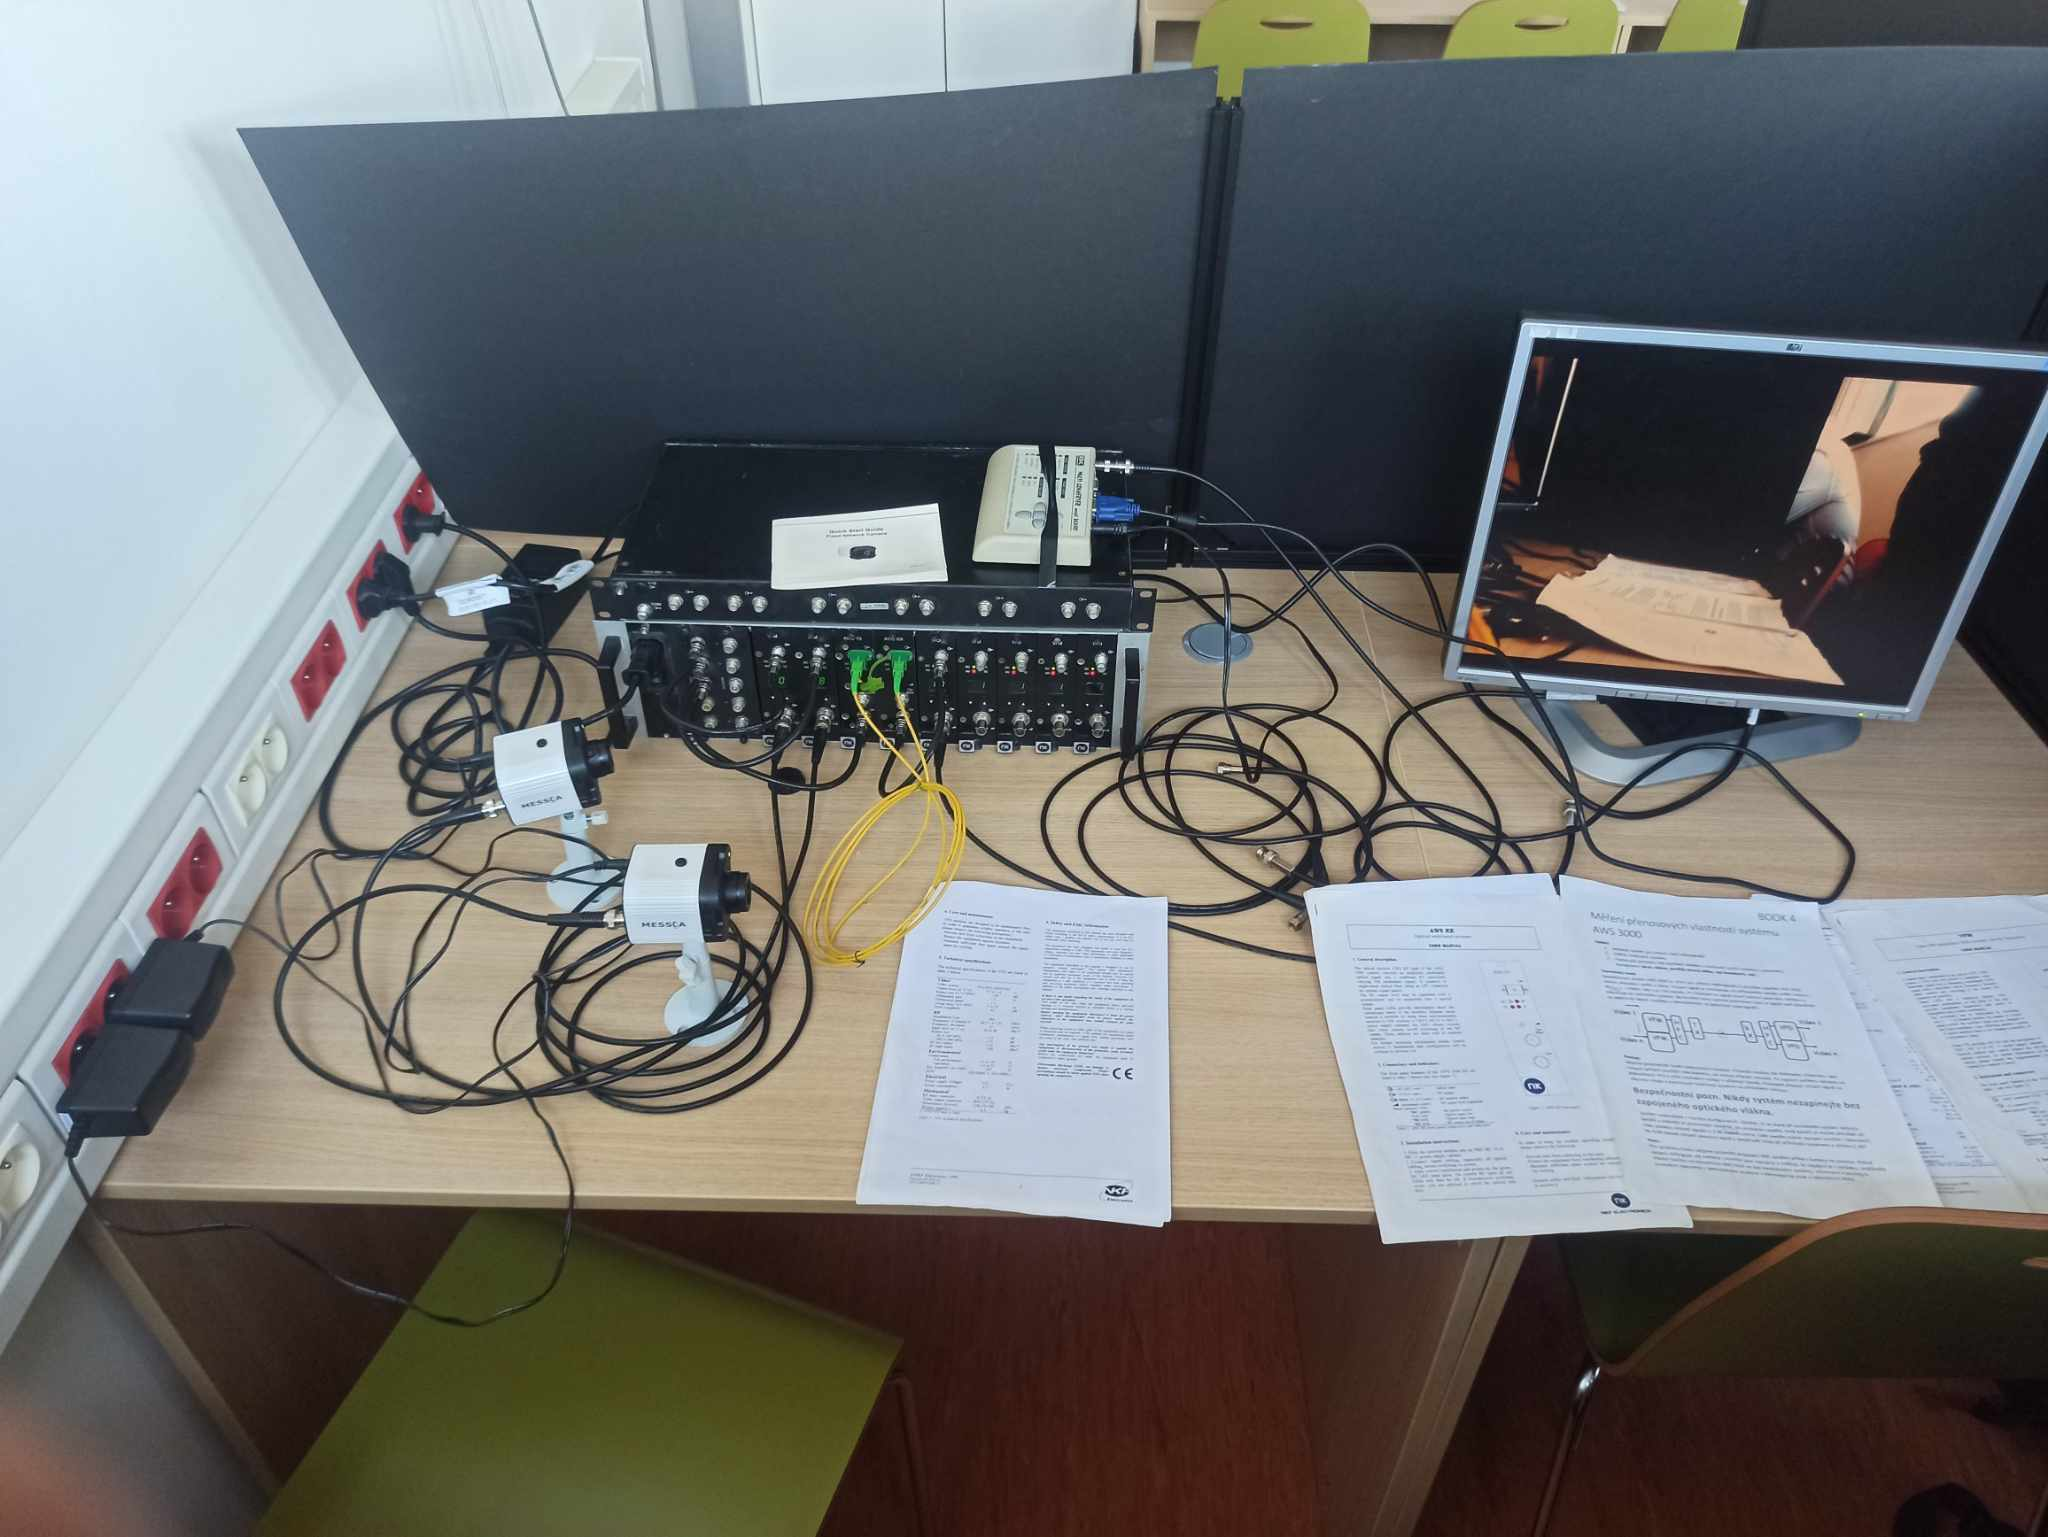
\includegraphics[width=0.58\textwidth]{text/img/ADS3000.jpg} 
    \caption{\label{fig:ADS} Sestavený systém}
\end{figure}

Audiosignál lze přenášet od \(20 [hz]\) do \(15 [kHz]\), při vyšších frekvencích dochází k nahodilému posunu fáze a k útlumu signálu.
Při nižších frekvencích dochází jen k výraznému útlumu.

RS232 lze provozovat do \(200 [kHz]\) a při vyšších frekvencích dochází k otočení fáze.
Rs232 má definovaný rozsah pro log jedničku \(3\) až \(15 [v]\) a log nulu \(-15\) až \(-3 [v]\). 
Na vstupu jsem posílal \(\pm 5\) a na výstupu četl \(\pm7\), což odpovídá standardu.


